\chapter{\xlabel{calib}SCUBA-2 data calibration}
\label{app:cal}

\section{\xlabel{fcf}Flux conversion factors (FCF)}
\label{app:fcf}

Primary and secondary calibrator observations have been reduced using
the specifically designed \file{dimmconfig\_bright\_compact.lis}.  The
maps produced from this are then analysed using tailor-made \picard\
recipes. For instructions on applying the FCFs to your map see
\cref{Section}{sec:cmult}{this page}.

A map reduced by the map-maker has units of pW. To calibrate the data
into units of janskys (Jy), a set of bright, point-source objects with
well-known flux densities are observed regularly to provide a flux
conversion factor (FCF). The data (in pW) can be multiplied by this
FCF to obtain a calibrated map. The FCF can also be used to assess the
relative performance of the instrument from night to night. The noise
equivalent flux density (NEFD) is a measure of the instrument
sensitivity, and while not discussed here, is also produced by the
\textsc{Picard} recipe shown here. For calibration of primary and
secondary calibrators, the FCFs and NEFDs have been calculated as
follows:

\begin{enumerate}
\item The \textsc{Picard} recipe \drrecipe{SCUBA2\_FCFNEFD} takes the
  reduced map, crops it, and runs background removal. Surface-fitting
  parameters are changeable in the \textsc{Picard} parameter file.

\item It then runs the \Kappa\ \beamfit\ task on the specified point
  source. The \task{beamfit} task will estimate the peak
  (uncalibrated) flux density and the FWHM. The integrated flux
  density within a given aperture (30-arcsec radius default) is
  calculated using \photom\ \autophotom. Flux densities for
  calibrators such as Uranus, Mars, CRL~618, CRL~2688 and HL~Tau are
  already known to \picard. To derive an FCF for other sources of
  known flux densities, the fluxes can be added to the parameter file
  with the source name (in upper case, spaces
  removed): \param{FLUX\_450.MYSRC~=~0.050}
  and \param{FLUX\_850.MYSRC~=~0.005} (where the values are in Jy),
  for example.

\item Three different FCF values are calculated:

  \begin{enumerate}

  \item \textbf{The Arcsecond (Aperture) FCF}
    \begin{equation}
      \label{eq:fcf_arcsec}
      \mathrm{FCF_{arcsec}} = \frac{S_{\mathrm{tot}}}{P_{\mathrm{int}} \times
        A_{\mathrm{pix}}}
    \end{equation}

    where $S_{\mathrm{tot}}$ is the total flux density of the
    calibrator, $P_{\mathrm{int}}$ is the integrated sum of the source
    in the map (in pW) and $A_{\mathrm{pix}}$ is the pixel area in
    arcsec$^2$, producing an FCF in Jy/arcsec$^2$/pW.

   \vspace{3mm}

  \item\textbf{The Beam (Peak) FCF}
    \begin{equation}
      \label{eq:fcf_beam}
      \mathrm{FCF_{beam}} = \frac{S_{\mathrm{peak}}}{P_{\mathrm{peak}}}
    \end{equation}
    producing an FCF in units of Jy/beam/pW. The measured peak signal here is 
    derived from the Gaussian fit of \task{beamfit}. The peak value is susceptible 
    to pointing and focus errors, and we have found this number to be somewhat unreliable,
    particularly at 450$\mu$m.
    
   \vspace{3mm}

  \item\textbf{The Beammatch FCF}
    This FCF is calculated in the same way as the Beam FCF decribed
    above, but after a matched filter is applied to the data (see Appendix \ref{app:mf}).
    This FCF is less commonly used than the former two types.

  \end{enumerate}

\end{enumerate}

For a true point source, the measured peak pixel in a map calibrated in units of Jy/beam 
(using the Beam FCF) is equivalent to the integrated total flux of the same source in a map 
calibrated in units of Jy/arcsec$^{2}$ (using the Arcsecond FCF). The ORAC-DR processing 
routine will automatically select the appropriate FCF based on the default data reduction recipe 
that was linked to your data at the time of observations. Note that the data reduction recipe can 
easily be changed when running ORAC-DR (see Section \ref{subsec:ChangeRecipe} for details).

\section{\xlabel{extinction}Extinction correction}

Starlink automatically applies the following multiplicative extinction correction to SCUBA-2 data:

\begin{equation}
\label{eq:extcor}
\mathrm{Extinction\:Correction} = \frac{1}{\mathrm{exp}[-\tau_{\nu}\times\mathrm{Airmass}]}
\end{equation}

Where $\tau_{\nu}$ is the opacity at the given frequency, $\nu$.

The atmospheric opacity at SCUBA-2’s operating frequencies are defined in 
terms of the opacity at 225 GHz. Optimizing the uniformity of the SCUBA-2 secondary 
calibrator fluxes as a function of atmospheric transmission has allowed calculation
of the atmospheric opacity relationships for the SCUBA-2 450\,$\mu$m and
850\,$\mu$m pass-bands to be determined. Full details of the analysis
and on-sky calibration methods of SCUBA-2 can be found in Dempsey et
al.\ (2013)~\cite{dempsey12}\cite{dempsey-spie} with
updated relations provided in Mairs et al.\ (2021)~\cite{mairs21}.

Archibald et al. (2002)\,\cite{archibald} describes how the Caltech
Submillimeter Observatory (CSO) 225\,GHz opacity, $\tau_{225}$,
relates to SCUBA opacity terms in each band, $\tau_{450}$ and
$\tau_{850}$. The JCMT water-vapour radiometer (WVM) uses the 183\,GHz
water line to calculate the precipitable water vapour (PWV) along the
line-of-sight of the telescope. This PWV is then input into an
atmospheric model to calculate the zenith opacity at 225\,GHz
($\tau_{225}$). Historically, this has allowed for ease of 
comparison with the adjacent CSO 225\,GHz tipping radiometer. 

The updated opacity relations (to be used in Equation \ref{eq:extcor}) 
derived by Mairs et al. (2021)~\cite{mairs21}
have been adopted as the default as of \textbf{Starlink release 2021A}:

\begin{equation}
\tau_{450} = 23.3 \times (\tau_{225} - 0.018 + 0.05\sqrt{\tau_{225}});
\end{equation}
and
\begin{equation}
\tau_{850} = 3.71 \times (\tau_{225} - 0.040 + 0.20\sqrt{\tau_{225}}).
\end{equation}

Previously, (\textbf{Starlink versions 2018A and before}) adopted as defaults the opacity relations 
found by Dempsey et al. (2013)~\cite{dempsey12}:

\begin{equation}
\tau_{450} = 26.0 \times (\tau_{225} - 0.012);
\end{equation}
and
\begin{equation}
\tau_{850} = 4.6 \times (\tau_{225} - 0.0043).
\end{equation}

The updated opacity relations as of Starlink release 2021A  will affect 
450 micron data obtained in very dry conditions and 850 micron data 
obtained in very dry or very wet conditions by up to 5\% (see Figure \ref{fig:NewExtCor}).

\textbf{Note that the default extinction corrections are intrinsically connected to the default FCFs
applied. If applying extinction corrections derived by Mairs et al. 2021 (\cite{mairs21}), the matching
FCFs must also be applied (see Appendix \ref{app:fcfs}). The ORAC-DR software assumes the Mairs et al 2021
results beginning in Starlink release 2021A. Starlink release 2018A and previous assume the 
Dempsey et al 2013~(\cite{dempsey12}) values by default.}

\begin{figure}
\begin{center}
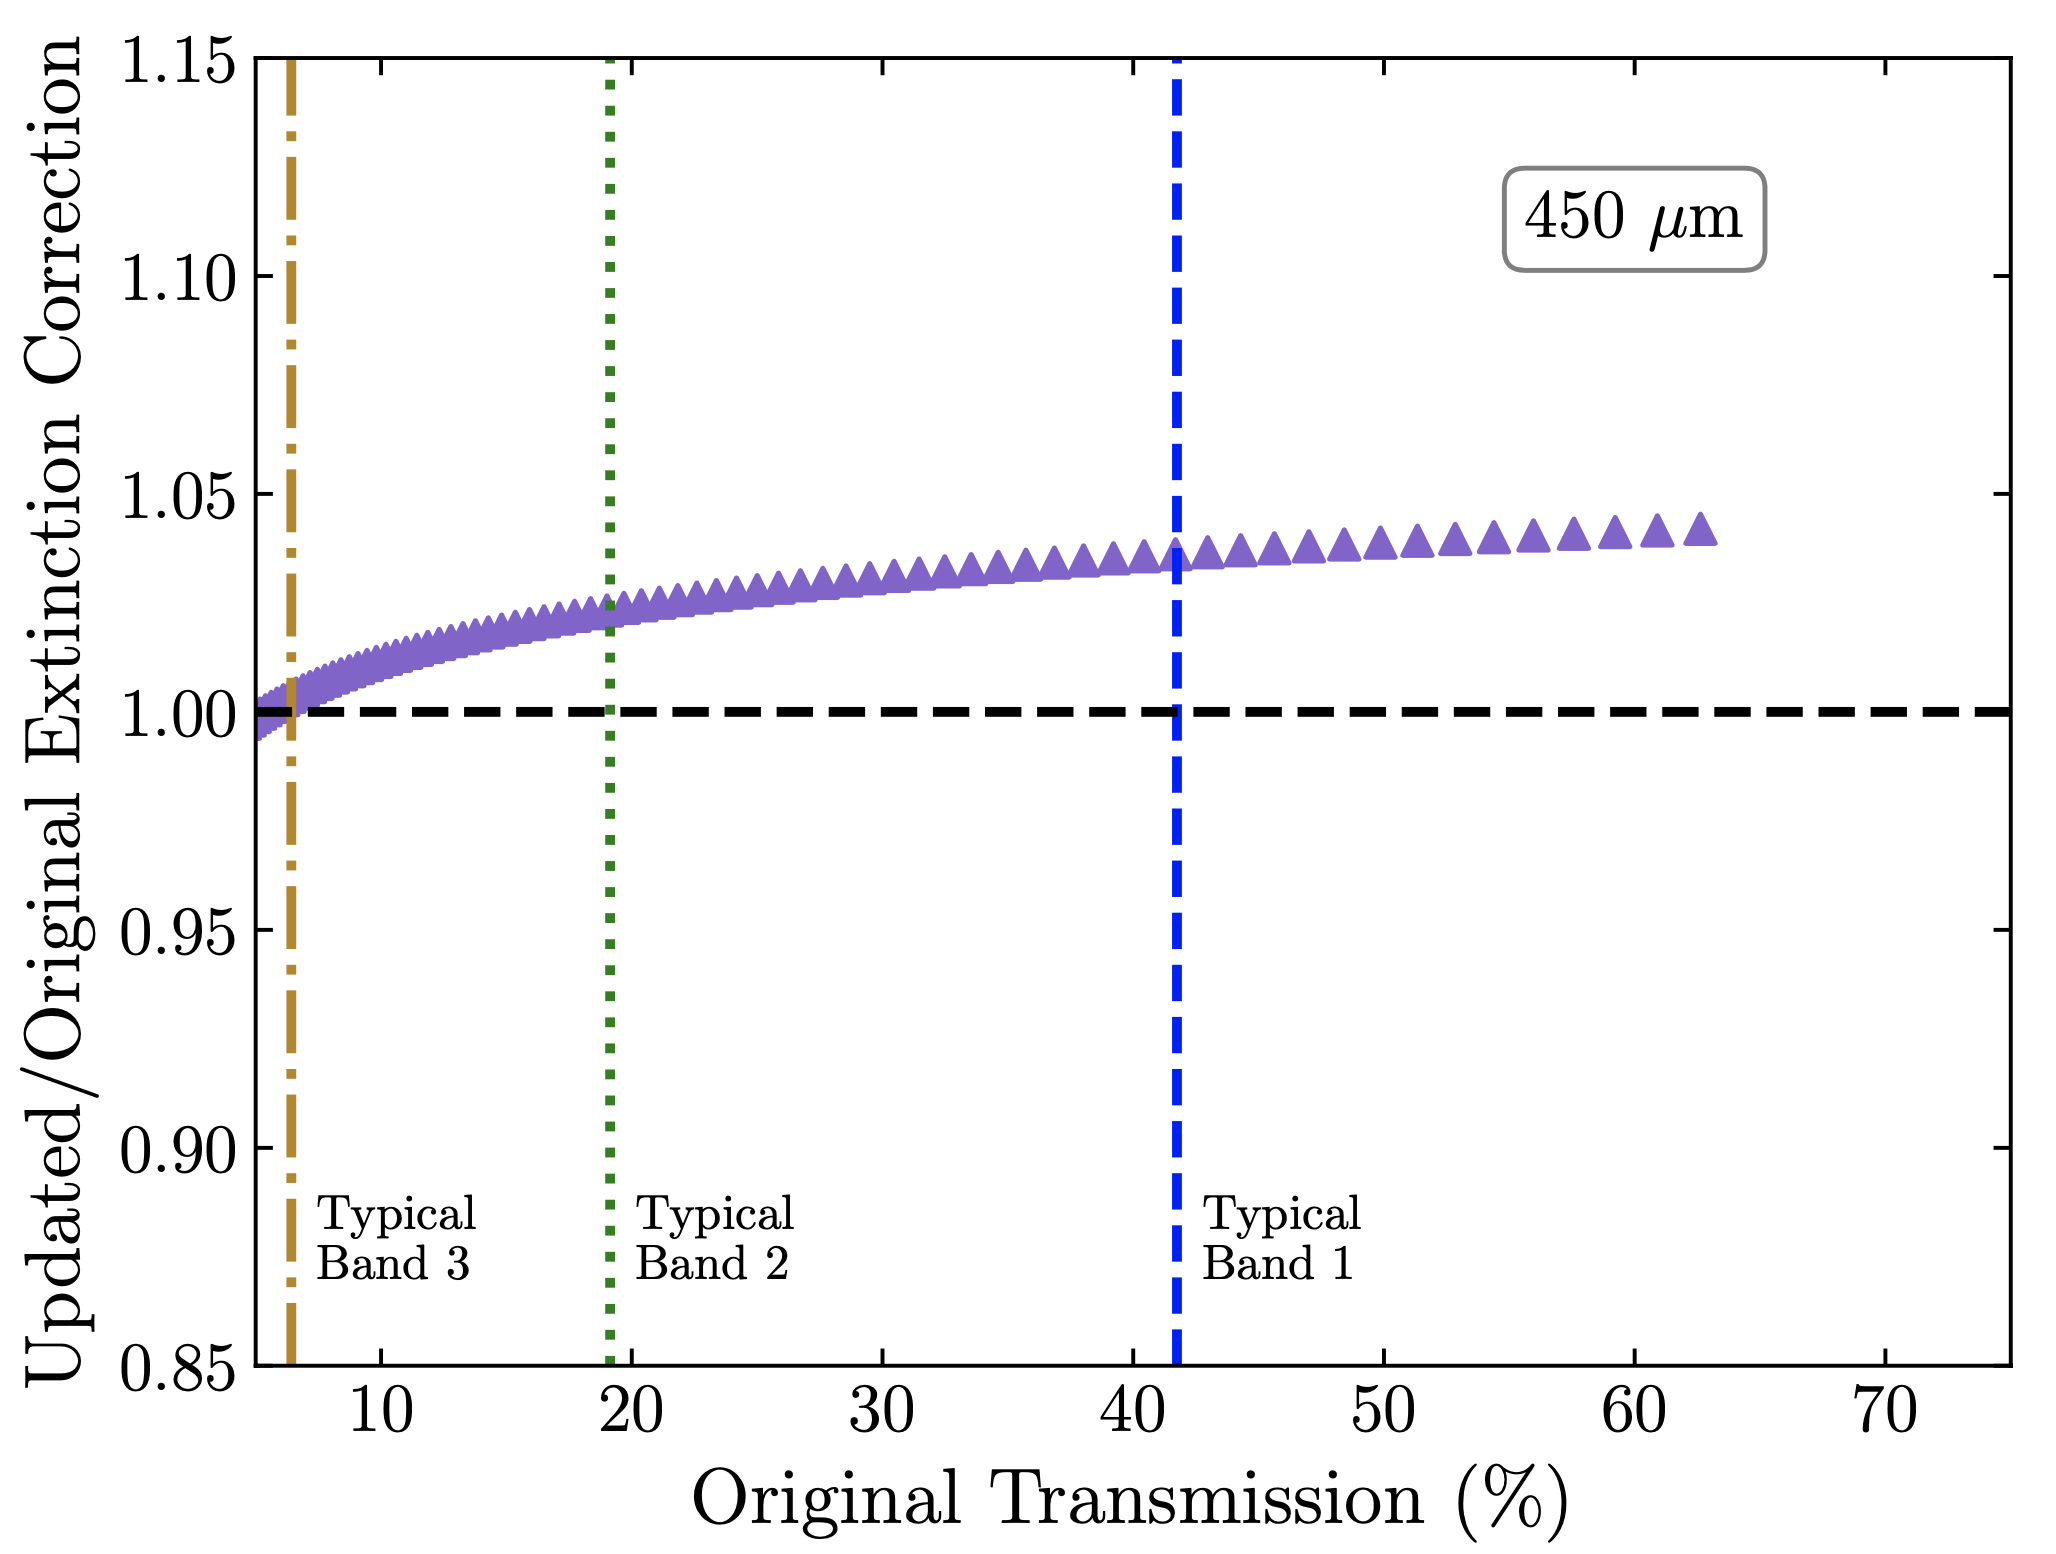
\includegraphics[width=0.4\linewidth]{sc21-NewExtCor-450} \hspace{0.02\linewidth}
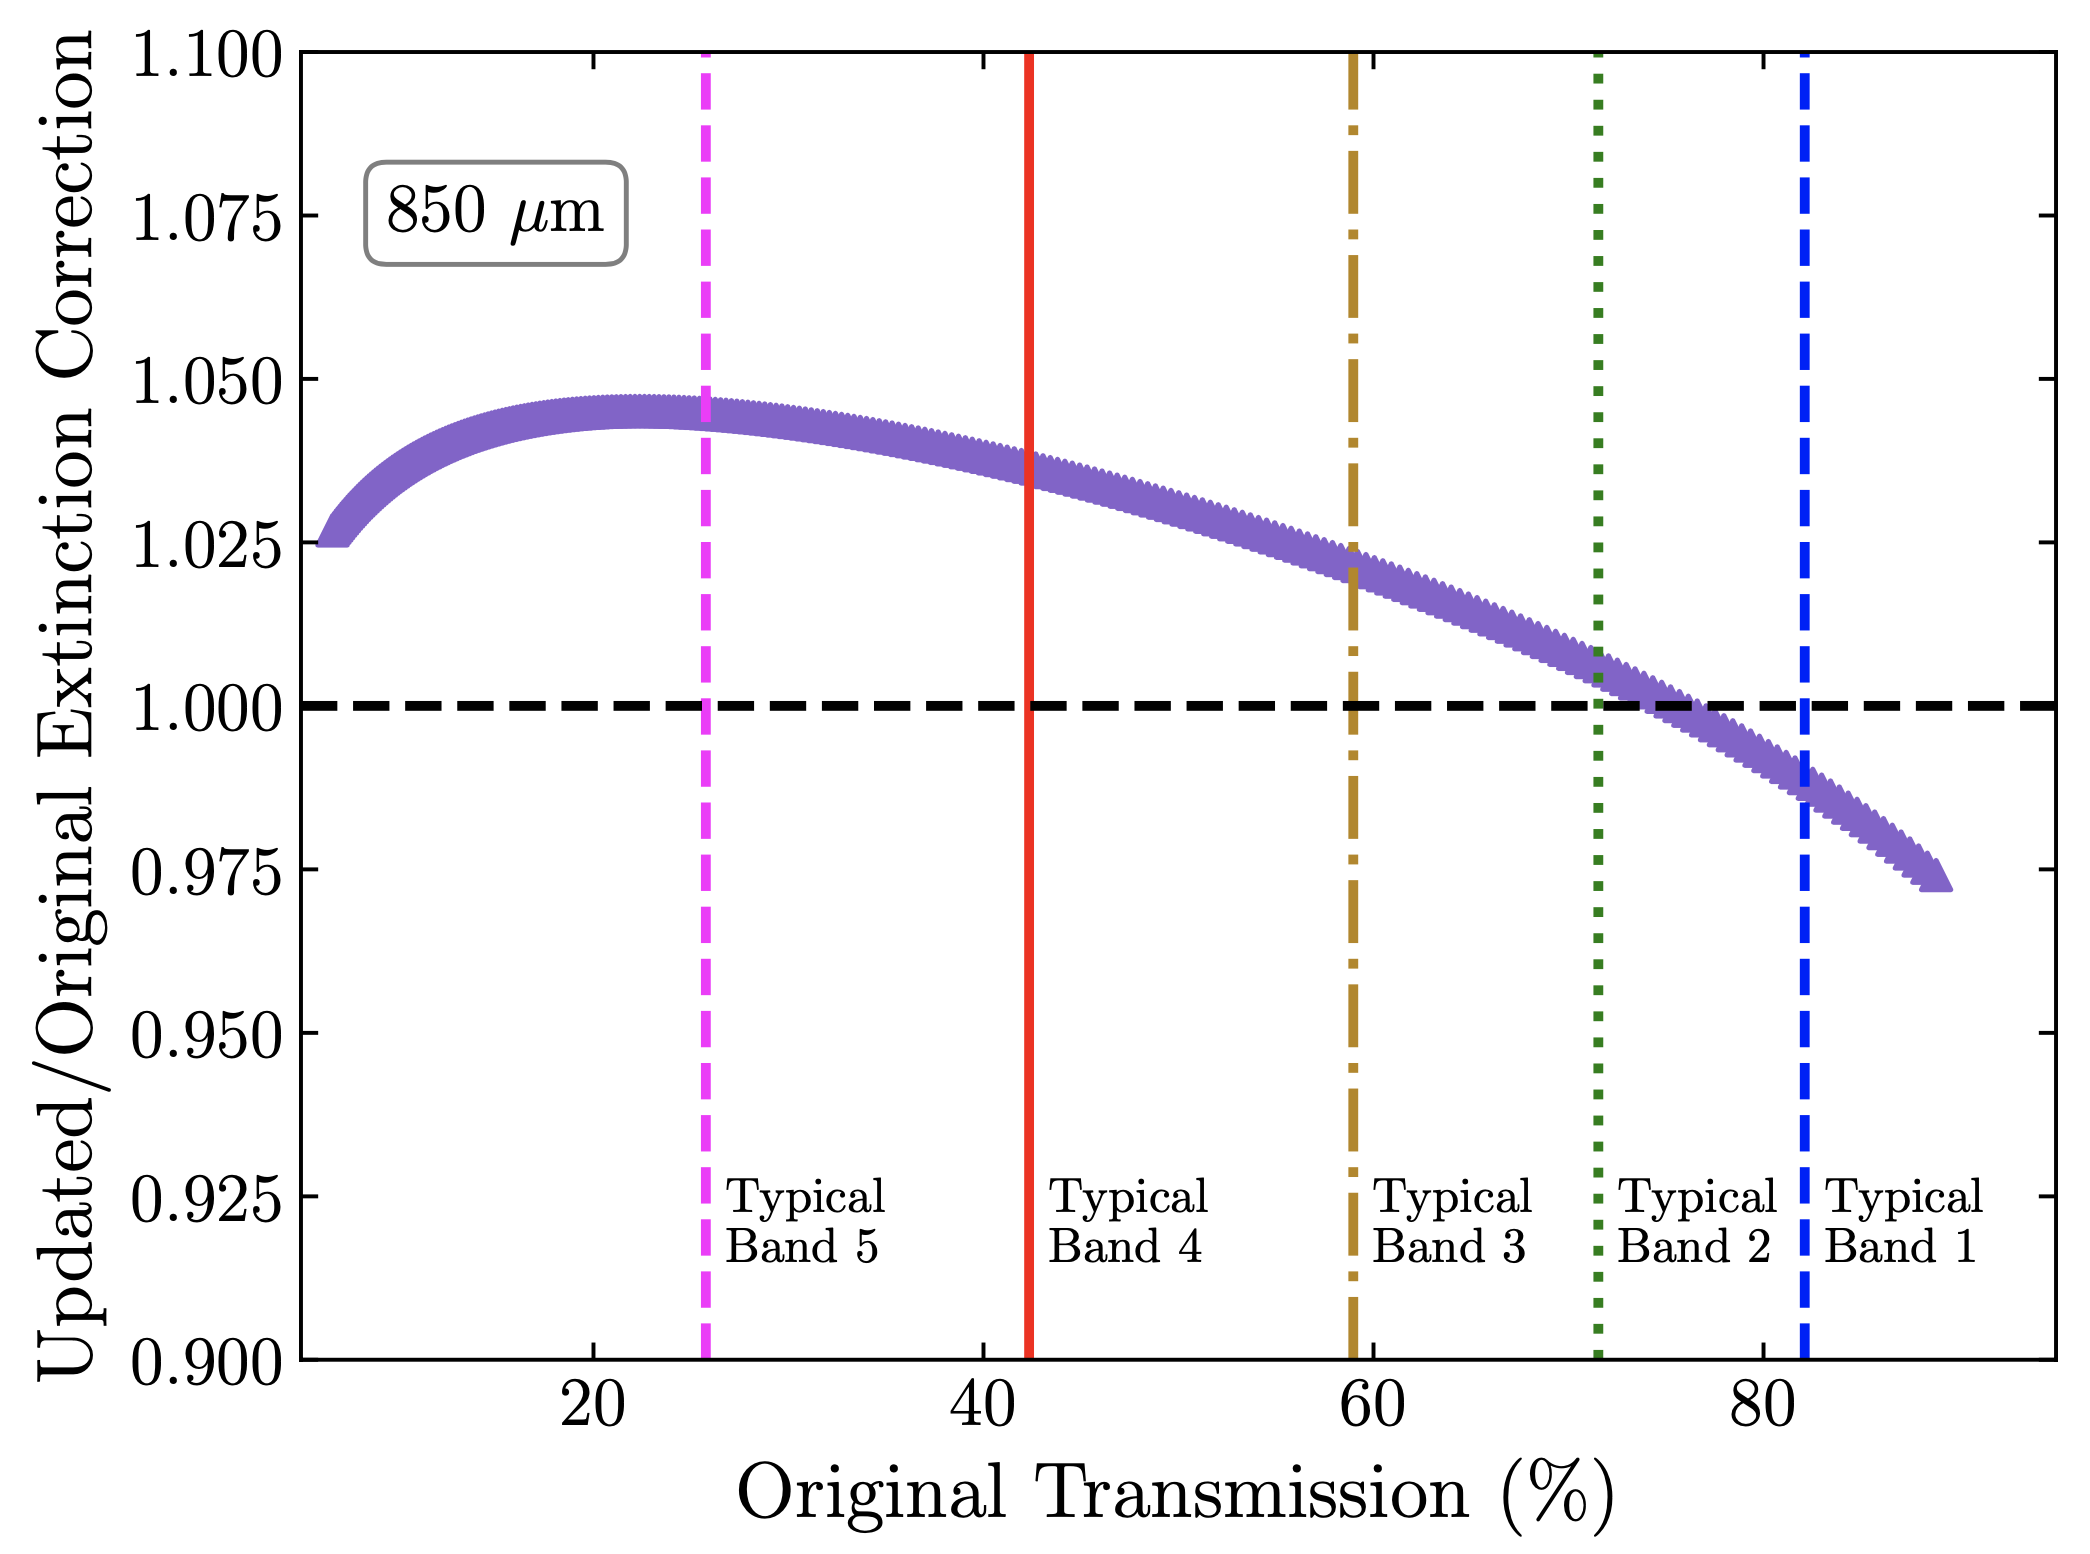
\includegraphics[width=0.4\linewidth]{sc21-NewExtCor-850}
\caption[Updated Extinction Corrections]{The new extinction corrections 
derived by Mairs et al (2021, \cite{mairs21}) divided by the original extinction corrections (Dempsey et al 2013~\cite{dempsey12}) 
as a function of atmospheric transmission. Vertical lines show the atmospheric transmission of the typical JCMT 
weather bands at each wavelength, assuming an airmass of 1.2. Left: 450 microns. Right: 850 microns. At 450 microns, 
the original correction is modified by a maximum of 5\% in very dry weather while at 850 micronas the original correction is 
modified by a maximum of 5\% in very dry or very wet conditions. The majority of 850 microns observations, however, require no modification to the original correction and less than 4\% of SCUBA-2 data is obtained in weather band 5. \label{fig:NewExtCor}}
\end{center}
\end{figure}


The SCUBA-2 filter characteristics are described in detail
\htmladdnormallinkfoot{on the JCMT
  website}{http://www.eaobservatory.org/jcmt/instrumentation/continuum/scuba-2/filters/}.

The extinction correction parameters that scale from $\tau_{225}$ to
the relevant filter have been added to the map-maker code. You can
override these values by setting \param{ext.taurelation.filtname} in
your map-maker config files to the three coefficients `($a$,$b$,$c$)' that
you want to use (following the form $\tau_{\nu} = a \times (\tau_{225} + b + c\sqrt{\tau_{225}})$), where \param{filtname} is the name of the
filter). The defaults are listed in
\file{\$SMURF\_DIR/smurf\_extinction.def}.

% It is worth noting that if an individual science map and
% corresponding calibrator observation has already been reduced with
% the old factors (and your source and calibrator are at about the
% same airmass and if the tau did not change appreciably), any errors
% in extinction correction should cancel out in the calibration.


